\documentclass[12pt]{beamer}
\usetheme{JuanLesPins}
\usecolortheme{spruce} 

\usepackage{ragged2e}
\usepackage[utf8]{inputenc}
\usepackage[brazil]{babel}
\usepackage[T1]{fontenc}
\usepackage{xcolor}
\usepackage{amsmath}
\usepackage{amsfonts}
\usepackage{amssymb}
\usepackage{graphicx}
\usepackage{setspace}
\setbeamertemplate{caption}[numbered]
\usepackage{hyperref}
\setbeamercovered{transparent} %transparente
%\setbeamertemplate{navigation symbols}{\includegraphics[width=0.2\linewidth]{Logo IFAM-CALMAT.png}}
\setbeamertemplate{navigation symbols}{}
\usepackage{tcolorbox}
\usepackage{colortbl}
\usepackage{xcolor}
\newcommand{\euler}{e}

\addtobeamertemplate{block begin}{}{\justifying}
\addtobeamertemplate{block alerted begin}{}{\justifying}
\addtobeamertemplate{block example begin}{}{\justifying}
\let\raggedright\justifying         
\AtBeginEnvironment{frame}{\justifying} 


\author[Joao Victor \& Everton de Souza]{% 
	Joao Victor\inst{1} \and Everton de Souza\inst{2}}
\title{Políticas educacionais para a Amazônia: teorias, práticas e contradições}
\institute[]{% 
	\textsuperscript{1,2} Graduando em Licenciatura em Matemática \\
}
\date{\today} 
\titlegraphic{
\includegraphics[width=0.4\textwidth]{imagens/logo.png}}

\begin{document}
	\onehalfspacing 
	
	\begin{frame}
		\titlepage
	\end{frame}
	
	\begin{frame}{Sumário}
		\tableofcontents
	\end{frame}
	
	\section{Resumo}
	
		\begin{frame}{Resumo}
			\begin{block}{Autores: Eraldo Carmo e Maria Prazeres (2015):}
				\begin{itemize}
					\item O artigo discute as configurações das políticas educacionais as populações do campo na Amazônia a partir da estrutura do Estado capitalista.
					
					\uncover<2->{
					\item O método de análise está assentado nas bases do materialismo histórico dialético a fim de compreender em que medida a lógica da racionalidade econômica que
					impera sobre tais políticas se reflete no direito à educação destas populações.
					}
				\end{itemize}
			\end{block}
		\end{frame}
		
		\begin{frame}{Resumo}
			\begin{block}{Autores: Eraldo Carmo e Maria Prazeres (2015):}
				\begin{itemize}
					\item Diante disso, se evidenciou os efeitos, desafios e contradições das políticas
					educacionais quando partem dos órgãos centrais para realidades específicas sem
					o conhecimento das heterogeneidades locais.
					
				\end{itemize}
			\end{block}
		\end{frame}
	
	\section{Fundamentos e Princípios}
		\begin{frame}{Políticas Públicas Educacionais}
			\begin{block}{Para Carmo e Prazeres (2015), temos:}
				\begin{itemize}
					\item Refletir sobre os princípios e as intencionalidades com que as políticas públicas se configuram no Estado é imprescindível para se entender a forma
					como são materializadas.
					
					\uncover<2->{
						\item Entretanto, não se pode perder de
						vista que as políticas públicas mudam no interior do Estado conforme a linha teórica do governo que estiver no poder.
					}
				\end{itemize}
			\end{block}
		\end{frame}
		
		\begin{frame}{Diferença entre Estado e governo}
			Höfling (2001) enfatiza:
			\begin{block}{Estado}
				\begin{itemize}
					\item Está solidificado na sociedade, seja através dos órgãos legislativos, tribunais, exército e outras;
					
					\uncover<2->{
					\item Representa o interesse de diferentes grupos sociais,
					principalmente dos setores econômicos.
					}
				\end{itemize}
			\end{block}
			
			\begin{block}{governo}
				\begin{itemize}
					\item É transitório;
					
					\uncover<2->{
					\item Representado por um partido que tem a oportunidade de imprimir seus programas e projetos na condução do Estado.
					}
				\end{itemize}
			\end{block}
		\end{frame}
		
			\begin{frame}{Diferença entre Estado e governo}
				\justifying
				Nessa perspectiva, Höfling (2001) apresenta que as concepções
				se modificam de acordo com a alternância de poder, o que se reflete na condução e elaboração das políticas sociais. \\
			\end{frame}
	
			\begin{frame}{Diferença entre Estado e governo}
				\justifying

				Para tanto, o Estado é demarcado por contradições sociais, culturais, políticas e econômicas. o governo que detém o poder, porém, busca reduzir estas contradições - que podem ser questionáveis - por meio das \textbf{políticas sociais}, principalmente para combater as desigualdades sociais.
			\end{frame}	
	
			\begin{frame}{Políticas Sociais}
				\justifying
		
				Para Höfling (ibidem), as políticas sociais se referem a ações que determinam o padrão de proteção social implementado pelo Estado, voltadas, em princípio, para a redistribuição dos benefícios sociais visando à diminuição das desigualdades estruturais produzidas pelo desenvolvimento socioeconômico.
			\end{frame}
	
			\begin{frame}{Políticas Sociais}
				\justifying
		
				As análises da autora reforçam os aspectos contraditórios do Estado, promovidos pelo modelo de desenvolvimento econômico. Entretanto, as políticas educacionais têm a função de reduzir os impactos negativos que atingem os setores menos favorecidos da sociedade.
			\end{frame}
	
			\begin{frame}{Políticas Públicas Educacionais}
				\justifying
				\begin{itemize}
				\item Tem-se questionado a forma como o Estado tem primado
				pela formulação das políticas públicas, uma vez que, na maioria das vezes, as decisões se dão de forma centralizada;
			
				\uncover<2->{
				\item Com isso, não são levadas em consideração os aspectos regionais, com suas especificidades, gerados no processo de implementação;
				}
			
				\uncover<3->{
				\item É impossível pensar Estado fora de um projeto político e de uma teoria social para a sociedade como um todo.
				}
				\end{itemize}
			\end{frame}
	
			\begin{frame}{Políticas Públicas Educacionais}
				\justifying
				\begin{itemize}
					
					\item No entendimento de Höfling (2001), a educação se reproduz conforme as concepções e ideologias do Estado.
					
					\uncover<2->{
					\item Por sua vez, como predominam os interesses
					capitalistas nos direcionamentos das ações estatais, as políticas educacionais não estão imunes a este processo.
					}
					
					\uncover<3->{
					\item Mesmo que o poder político do Estado seja
					assumido por governos de diferentes vertentes ideológicas, a essência das políticas se mantém, uma vez que não rompem com a lógica do capital.
					}
				\end{itemize}
			\end{frame}
			
			\begin{frame}{Políticas Públicas Educacionais}
				\justifying
				O Estado capitalista atua como guardião dos direitos dos cidadãos,
				porém, em função da manutenção dos seus poderes; ou seja, é mais com a
				intenção de promover a dominação do que de conferir autonomia aos sujeitos.
				Nessa perspectiva, as políticas sociais são implementadas como forma de regular
				os conflitos sociais.
			\end{frame}
			
			\begin{frame}{Políticas Públicas Educacionais}
				\justifying
				
				Notadamente no campo do discurso, a educação está sempre em
				evidência na agenda governamental como estratégia fundamental, seja em relação
				ao aspecto econômico ou como indutora do desenvolvimento e no combate
				às desigualdades sociais.
			\end{frame}
			
			\begin{frame}{Políticas Públicas Educacionais}
				\justifying
				
				Como se verifica, as políticas não são formuladas para atender toda a
				população, mas um público específico, com o propósito de amenizar determinados
				impactos sociais. Isso evidencia seu caráter reducionista e compensatório, como
				bem destacaram Oliveira e Ferreira (2008).
			\end{frame}
			
			\begin{frame}{Políticas Públicas Educacionais}
				\begin{itemize}
					\item O setor privado passou a exercer grandes influências nos direcionamentos
					das políticas educacionais. Para esses novos sujeitos, o Estado deveria ser mais
					eficiente em suas ações; com isso, a função pública assumiu novos contornos
					como normalizadora, reguladora e avaliadora (OLIVEIRA; FERREIRA, 2008).
					
					\uncover<2->{
					\item Implantação do
					Censo Escolar, do Sistema de Avaliação da Educação Básica (SAEB), do Exame
					Nacional do Ensino Médio (ENEM) e do Exame Nacional de Cursos (Provão)
					(SHIROMA, 2000).
					}
				\end{itemize}
			\end{frame}
			
			\begin{frame}{Políticas Públicas Educacionais}
				\justifying
				
				Há uma grande preocupação com os dados quantitativos em detrimento do qualitativo. Portanto,
				a educação, com base nas reformas, realinhou-se às estratégias das políticas de
				cunho compensatório. O Estado consolidou esses novos reordenamentos a fim de atender à
				demanda do capital em detrimento dos direitos sociais da população.
			\end{frame}
			
			\begin{frame}{Políticas Públicas Educacionais}
				\begin{itemize}
					\item Para o governo, a política de fundos (FUNDEF/FUNDEB) para financiar o Ensino Fundamental
					e, posteriormente, a Educação Básica, representaria mais recursos para a
					educação.
					
					\uncover<2->{
						\item Todavia, na prática, configurou-se mais como um jogo contábil do que
						propriamente novas fontes de recursos para a educação.
					}
					
					\uncover<3->{
					\item Isso porque o fundo
					apenas centralizou a capitalização dos impostos destinados à educação da União,
					Estados e municípios, fazendo com que houvesse a redistribuição com base no
					número de matrículas dos sistemas de ensino.
					}
				\end{itemize}
			\end{frame}
			
			\begin{frame}{Políticas Públicas Educacionais}
				\justifying
				
				Concretamente, tanto o FUNDEF quanto o FUNDEB não significaram
				novas fontes de financiamento, uma vez que mantiveram os mesmos percentuais
				de aplicação na educação, conforme orienta a Constituição Federal de 1988: o
				mínimo de 25\% da receita para Estados e municípios e, para a União, 18\%.
			\end{frame}
			
			\begin{frame}{Políticas Públicas Educacionais}
				\justifying
				
				Para Boneti (2011), cada momento histórico produz, no contexto da inter-relação entre a produção
				econômica, cultura e interesses dos grupos dominantes, ideologias a partir
				das quais verdades relativas tornam-se absolutas. E essas observações contribuem para compreender o momento
				econômico do país nos anos de 1990.
			\end{frame}
		
	\section{Desafios e Contradições}
	
		\begin{frame}{Políticas Públicas Educacionais}
			\begin{itemize}
				\item Discutir a construção de políticas públicas no Estado, partindo do local, é romper com lógica da centralização e concentração, que ainda permanece,
				principalmente no campo da educação na qual as definições se dão no governo
				central, cabendo aos estados e municípios a execução.
				
				\uncover<2->{
					\item Mesmo que haja um ou outro ente federado que tenha programas
					e projetos específicos elaborados por seus respectivos governos, estes não
					podem, no campo da legislação, definir leis que se sobreponham à LDB.
				}
				
			\end{itemize}
		\end{frame}
		
		\begin{frame}{Políticas Públicas Educacionais}
			\justifying
			
			Existe a tendência de alguns povos, sobretudo os considerados desenvolvidos,
			de adotarem o entendimento segundo o qual as suas sociedades centralizam a
			verdade em termos de costumes culturais, desenvolvimento social e econômico,
			etc. Estas sociedades têm dificuldade de compreender como verdade as diferenças
			culturais que não sejam as suas.
		\end{frame}
		
		\begin{frame}{Políticas Públicas Educacionais}
			\justifying
			
			Essas concepções se refletem em certa imposição pelo Estado na forma de organização das escolas do campo no território da Amazônia. Neste aspecto, encontram-se escolas multisseriadas, que, embora estejam presentes em todos os sistemas de ensinos dos Estados da federação, têm predominância nas regiões norte e nordeste do país.
		\end{frame}
		
		\begin{frame}{O multisseriado no estado do Amazonas}
			\justifying
			Conforme Ferreira, Andrade e Nascimento (2025),
			\begin{itemize}
				\item O  ensino  multisseriado  caracteriza-se  pela  reunião  de  estudantes  de diferentes  séries/anos  em  um  mesmo  espaço  escolar,  ou  seja,  em  uma  única turma sob a responsabilidade de um único professor ou professora.
				
				
				\uncover<2->{
				\item Esse modelo organizacional está presente, sobretudo, em áreas rurais   do   país,   onde   atualmente   existem   69.248   turmas   multisseriadas (OBECAS/INEP, 2025). A Região Norte concentra a maior incidência desse tipo de organização escolar.
				}
			\end{itemize}
		\end{frame}
		
		\begin{frame}{Políticas Públicas Educacionais}
			\justifying
			
			A precarização do ensino nas escolas multisseriadas é promovida pela
			negligência do próprio poder público, uma vez que é o principal agente de
			implementação das políticas educacionais. Para o Estado, as escolas multisseriadas
			são problema, ao invés de ser a solução da oferta do ensino às populações do
			campo na Amazônia em função da dispersão geográfica em que vivem. 
		\end{frame}
		
		\begin{frame}{Políticas Públicas Educacionais}
			\justifying
			
			 Nos últimos anos, a forma que o Estado encontrou para eliminar as escolas multisseriadas no campo foi apoiar os municípios para realizarem a nucleação. Cuja classifação pelo Instituto Nacional de Estudos e Pesquisas Educacionais Anísio Teixeira (INEP) é “procedimento político-administrativo que consiste na reunião de várias escolas isoladas em uma só, desativando ou demolindo as demais”
		\end{frame}
		
		\begin{frame}{Políticas Públicas Educacionais}
			\justifying
			
			Nos últimos anos, a forma que o Estado encontrou para eliminar as escolas multisseriadas no campo foi apoiar os municípios para realizarem a nucleação. Cuja classifação pelo Instituto Nacional de Estudos e Pesquisas Educacionais Anísio Teixeira (INEP) é “procedimento político-administrativo que consiste na reunião de várias escolas isoladas em uma só, desativando ou demolindo as demais”
		\end{frame}
		
		\begin{frame}{Políticas Públicas Educacionais}
			\justifying
			
			A pesquisa de mestrado \textit{O fechamento das escolas multisseriadas no Amazonas - (UFAM)} resultou na hipótese de tese que sustenta que no Amazonas, o fechamento das escolas multisseriadas alinha-se a internacionalização da Amazônia; nega os processos formativos, acentua a desigualdade social e potencializa aprivatização do transporte escolar; por consequência, a mediação entre capital e trabalho,é a nucleação das escolas.
		\end{frame}
		
		\begin{frame}{O multisseriado no estado do Amazonas}
			\justifying
			Conforme Ferreira, Andrade e Nascimento (2025),
			\begin{itemize}
				\item Entretanto,   essa   necessidade   histórica   tem   sido   frequentemente invisibilizada pelas políticas públicas contemporâneas, que tendem a associar a multisseriação  a  atraso  ou  precariedade. 
				
				
				\uncover<2->{
					\item Esse  enquadramento  contribui  para processos de desmonte do ensino no campo, evidenciados pelos altos índices de  fechamento  de  escolas.
				}
			\end{itemize}
		\end{frame}
		
		\begin{frame}{O multisseriado no estado do Amazonas}
			\justifying
			Conforme Ferreira, Andrade e Nascimento (2025),
			\begin{itemize}
				\item Entre  1997  e  2018,  foram  extintas  milhares  de instituições  rurais  em  todo  o  país  (Taffarel,  Costa  e  Júnior,  2020).  
				
				
				\uncover<2->{
					\item Mais recentemente, entre 2000 e2023, contabilizou-se o fechamento de mais de 160 mil  escolas,  sendo  109  mil  apenas  em  áreas  rurais.
				}
			
			
				\uncover<3->{
				\item No  Amazonas,  esse fenômeno  também  se  fez  presente,  representando  uma  ameaça  ao  direito  à educação em comunidades distantes.
				}
			\end{itemize}
		\end{frame}
		
		\begin{frame}{O multisseriado no estado do Amazonas}
			\justifying
			
			Dentre  os  62  municípios  do  estado  do  Amazonas,  São  Gabriel  da Cachoeira destaca-se por concentrar o maior número de escolas multisseriadas do  campo,  com  192  unidades,  evidenciando  sua  importância  estratégica  na oferta educacional em territórios rurais e ribeirinhos Amazônicos (Mapa 1).
			
			$$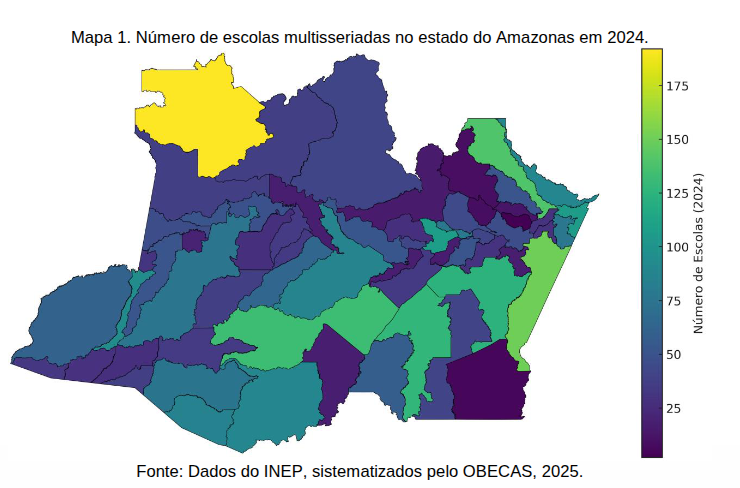
\includegraphics[scale=0.2]{imagens/obeca.png}$$
		\end{frame}
		
		\begin{frame}{Políticas Públicas Educacionais}
			\justifying
			Para Boneti (2011), os princípios do etnocentrismo têm orientado as decisões
			do Estado na definição das políticas públicas. Assim, a substituição das escolas
			multisseriadas pelas seriadas com a constituição das escolas núcleos, obedeceria
			essa lógica de organização do ensino como a mais apropriada para a oferta da
			educação às populações do campo.
		\end{frame}
		
		
	\section{Algumas Impressões}
	
		\begin{frame}{Políticas Públicas Educacionais}
			\begin{itemize}
				\item As políticas educacionais elaboradas sob a vertente do Estado capitalista
				têm ignorado a participação da sociedade; com isso, predominam os interesses
				dos governos que estão no poder.
				
				\uncover<2->{
				\item Nessa perspectiva, prevalece o caráter da
				homogeneidade na concepção das políticas em detrimento da heterogeneidade,
				como é caso da Amazônia.}
				
				\uncover<3->{
				\item Nesse aspecto, as escolas multisseriadas são um
				problema na estrutura educacional dos sistemas de ensino para os governos.}
			\end{itemize}
		\end{frame}
		
		\begin{frame}{Políticas Públicas Educacionais}
			\begin{itemize}
				\item Entretanto, contraditoriamente, para as populações do campo são uma
				forma de garantir a educação nos locais em que residem.
				
				\uncover<2->{
					\item Nesse contexto, o
					desafio é o Estado reconhecer essas especificidades a fim de estruturar políticas
					educacionais elaboradas de forma contextualizada.}
			\end{itemize}
		\end{frame}
		
	\section{Perguntas para reflexão}
	
		\begin{frame}{Perguntas para discussão}
			\begin{block}{Sobre a Autonomia das Políticas Locais}
				\justifying
				Como a distinção entre Estado (permanente) e Governo (transitório) afeta a continuidade das políticas educacionais na Amazônia, considerando que o governo federal centraliza recursos e legislação, deixando estados e municípios com apenas uma "autonomia relativa"?
			\end{block}
		\end{frame}
		
		\begin{frame}{Perguntas para discussão}
			\begin{block}{Sobre a Influência Internacional}
				\justifying
				Até que ponto o direito à educação na região é condicionado por ajustes econômicos de órgãos como o Banco Mundial e o FMI, que priorizam o custo-benefício e a redução de gastos sociais?
			\end{block}
		\end{frame}
		
		\begin{frame}{Perguntas para discussão}
			\begin{block}{Sobre a Efetividade do Financiamento}
				\justifying
				Se o FUNDEF e o FUNDEB são vistos como um "jogo contábil" que apenas redistribui impostos sem criar novas fontes de recursos, como garantir a universalização do ensino em uma região onde os custos logísticos são naturalmente mais elevados?
			\end{block}
		\end{frame}
		
		\begin{frame}{Perguntas para discussão}
			\begin{block}{Sobre a Autonomia das Políticas Locais}
				\justifying
				Como a distinção entre Estado (permanente) e Governo (transitório) afeta a continuidade das políticas educacionais na Amazônia, considerando que o governo federal centraliza recursos e legislação, deixando estados e municípios com apenas uma "autonomia relativa"?
			\end{block}
		\end{frame}
		
		\begin{frame}{Perguntas para discussão}
			\begin{block}{Sobre o Etnocentrismo Pedagógico}
				\justifying
				A imposição de modelos urbanos e a desqualificação dos saberes locais podem ser consideradas uma forma de etnocentrismo, onde o Estado trata a sociodiversidade amazônica como algo a ser "corrigido" por padrões de centros desenvolvidos?
			\end{block}
		\end{frame}
		
		\begin{frame}{Perguntas para discussão}
			\begin{block}{Sobre a Realidade das Escolas Multisseriadas}
				\justifying
				Diante dos dados de fechamento de milhares de escolas rurais no Amazonas, a nucleação (reunir alunos em sedes centrais) realmente garante o direito à educação ou acaba por precarizar o acesso de populações ribeirinhas e dispersas?
			\end{block}
		\end{frame}
		
		\begin{frame}{Perguntas para discussão}
			\begin{block}{Sobre a Participação Social}
				\justifying
				Como superar a centralização das decisões para que as políticas deixem de ser impostas "de cima para baixo" e passem a ser construídas com a participação efetiva e o reconhecimento das especificidades das populações amazônidas?
			\end{block}
		\end{frame}
		
		
	\section{Referências}
	
		\begin{frame}{Referências}
			\begin{itemize}
				\small
				\item DO CARMO, Eraldo Souza. Políticas educacionais para a Amazônia: teorias, práticas e contradições. Revista Brasileira de Política e Administração da Educação-Periódico científico editado pela ANPAE, 2022.
				
				\item DA SILVA FERREIRA, Jarliane; DE ANDRADE, Patrício Freitas; NASCIMENTO, Greicy Oliveira. O multisseriado no estado do Amazonas: indicadores, políticas e reflexões. Caderno Pedagógico, v. 22, n. 12, p. e20904-e20904, 2025.
				
				\item UCHOA, Iraci Carvalho; MOURÃO, Arminda Rachel Botelho; MOURA, Edilberto Santos. O fechamento das escolas multisseriadas no Amazonas. Revista Educação e Políticas em Debate, v. 12, n. 1, p. 174-184, 2023.
			\end{itemize}
		\end{frame}
		


	
	
	
	
\end{document}